% Domineering: rules, examples and the theory behind it.
% Build: xelatex domineering.tex (twice).  All values were computed with CGSuite 2.1.1.
\documentclass[11pt,a4paper]{article}
\usepackage[margin=2.3cm]{geometry}
\usepackage{fontspec}
\usepackage{unicode-math}
\setmainfont{LibertinusSerif}[Extension=.otf, UprightFont=*-Regular, BoldFont=*-Bold,
  ItalicFont=*-Italic, BoldItalicFont=*-BoldItalic]
\setsansfont{LibertinusSans}[Extension=.otf, UprightFont=*-Regular, BoldFont=*-Bold, ItalicFont=*-Italic]
\setmathfont{LibertinusMath-Regular.otf}
\usepackage{tikz}
\usepackage{booktabs}
\usepackage{array}
\usepackage{enumitem}
\usepackage{caption}
\usepackage{float}
\usepackage[most]{tcolorbox}
\usepackage{titlesec}
\usepackage{fancyhdr}
\usepackage[hidelinks]{hyperref}

\definecolor{leftc}{HTML}{2F5FD0}   % Left = vertical = blue
\definecolor{rightc}{HTML}{D23C3C}  % Right = horizontal = red
\definecolor{gridc}{HTML}{9AA0AA}
\definecolor{boxbg}{HTML}{F3F5FA}
\definecolor{boxrule}{HTML}{C9D1E3}

\titleformat{\section}{\Large\sffamily\bfseries}{\thesection}{0.6em}{}
\titleformat{\subsection}{\large\sffamily\bfseries}{\thesubsection}{0.6em}{}
\setlist{itemsep=2pt, topsep=4pt}
\captionsetup{font=small, labelfont=bf}
\pagestyle{fancy}
\fancyhf{}
\fancyhead[L]{\small\sffamily Domineering}
\fancyhead[R]{\small\sffamily\thepage}
\renewcommand{\headrulewidth}{0.3pt}

\newtcolorbox{keybox}[1][]{colback=boxbg, colframe=boxrule, boxrule=0.6pt, arc=2pt,
  left=8pt, right=8pt, top=6pt, bottom=6pt, fonttitle=\sffamily\bfseries,
  coltitle=black, colbacktitle=boxrule, #1}

% ---------------------------------------------------------------- board drawing
% Row r (1 = top), column c (1 = left).  Cell (r,c) spans x in [c-1,c], y in [-r,-r+1].
\newcommand{\grid}[2]{\draw[gridc, line width=0.5pt] (0,0) grid (#2,-#1);}
\newcommand{\sq}[2]{\draw[gridc, line width=0.5pt] ({#2-1},{-#1}) rectangle ({#2},{-#1+1});}
\newcommand{\vd}[2]{\fill[leftc, rounded corners=1.5pt]
  ({#2-1+0.13},{-#1-1+0.13}) rectangle ({#2-0.13},{-#1+1-0.13});}
\newcommand{\hd}[2]{\fill[rightc, rounded corners=1.5pt]
  ({#2-1+0.13},{-#1+0.13}) rectangle ({#2+1-0.13},{-#1+1-0.13});}
\newcommand{\lab}[3]{\node[font=\sffamily\bfseries\small, text=black!65] at ({#2-0.5},{-#1+0.5}) {#3};}
\newcommand{\dm}{\mathbin{\vert}}  % separator in {L | R}
\newcommand{\game}[2]{\{\,#1 \dm #2\,\}}

\title{\sffamily\bfseries Domineering\\[2pt]
  \large\mdseries How the game works, and the mathematics behind it}
\author{}
\date{\small November 2026 \textperiodcentered{} all values computed with CGSuite 2.1.1}

\begin{document}
\maketitle
\thispagestyle{fancy}

\begin{keybox}[title=In one paragraph]
Two players take turns placing dominoes on a grid.  \textcolor{leftc}{\textbf{Left}} always
places hers \textcolor{leftc}{\textbf{vertically}}, \textcolor{rightc}{\textbf{Right}} always places his
\textcolor{rightc}{\textbf{horizontally}}.  A domino covers two empty adjacent squares.  The first player
who cannot place a domino \textbf{loses}.  There is no luck, no hidden information and no draw.
As play goes on the board falls apart into separate regions, and combinatorial game theory
assigns each region a \emph{value}.  Adding the values tells you who wins and how.
\end{keybox}

\section{Rules}

\begin{itemize}
  \item The board is a rectangular grid, usually $8\times 8$.  It may have holes, and any set of
        squares works.
  \item \textbf{Left} (blue) places a domino \emph{vertically}: it covers a square and the square
        directly below it.  \textbf{Right} (red) places a domino \emph{horizontally}: it covers a
        square and the square to its right.
  \item Dominoes may not overlap or stick out of the board.  Players alternate; either may start.
  \item \textbf{A player who has no legal move on their turn loses} (\emph{normal play}).
\end{itemize}

\begin{figure}[h]
\centering
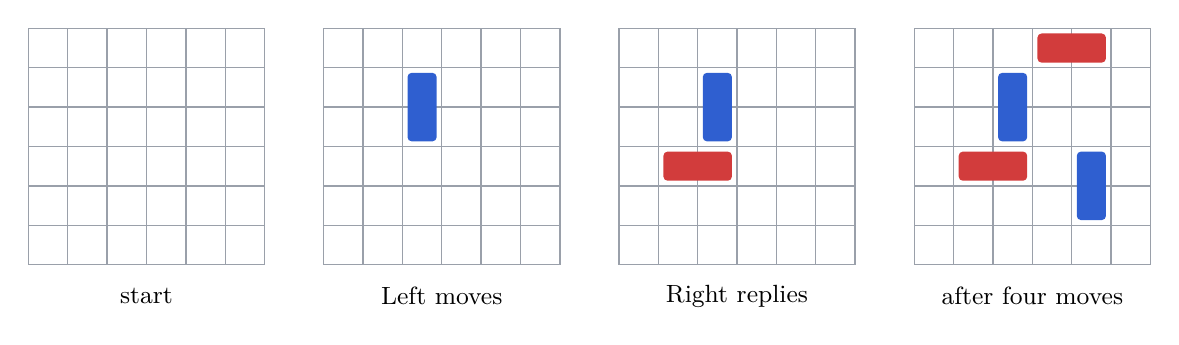
\begin{tikzpicture}[scale=0.5]
  \begin{scope}
    \grid{6}{6}
    \node[font=\small] at (3,-6.8) {start};
  \end{scope}
  \begin{scope}[xshift=7.5cm]
    \grid{6}{6} \vd{2}{3}
    \node[font=\small] at (3,-6.8) {Left moves};
  \end{scope}
  \begin{scope}[xshift=15cm]
    \grid{6}{6} \vd{2}{3} \hd{4}{2}
    \node[font=\small] at (3,-6.8) {Right replies};
  \end{scope}
  \begin{scope}[xshift=22.5cm]
    \grid{6}{6} \vd{2}{3} \hd{4}{2} \vd{4}{5} \hd{1}{4}
    \node[font=\small] at (3,-6.8) {after four moves};
  \end{scope}
\end{tikzpicture}
\caption{An opening on a $6\times6$ board.  Blue dominoes are Left's (vertical), red ones Right's
(horizontal).}
\end{figure}

The game was invented by Göran Andersson around 1973.  It was popularised as
\emph{Crosscram} in Martin Gardner's \emph{Scientific American} column in 1974, and it is
one of the central examples in \emph{Winning Ways} by Berlekamp, Conway and Guy.

\paragraph{Who is favoured?}  The two players are not symmetric on a rectangle.  A board that is
wide gives Right more room for horizontal dominoes, and a tall board helps Left.  On a square
board the player who moves first usually has the edge.  Section~\ref{sec:boards} gives exact
results.

\section{Thinking in regions}

Every domino splits the empty squares further.  After a few moves the board is a collection of
\emph{separate regions}, and a move in one region never affects another.  On each turn a player
chooses \emph{one} region and moves there.  This is a \emph{disjunctive sum} of games.  The key
fact of combinatorial game theory is that every region has a \textbf{value} $G$, and the values
of the regions simply \textbf{add up}.

\subsection{\texorpdfstring{The notation $\{\,L \mid R\,\}$}{The notation {L | R}}}

A position is written $\game{L}{R}$, where $L$ lists the values Left can move to and $R$ the
values Right can move to.  Positive values favour Left, negative values favour Right:

\begin{center}
\begin{tabular}{@{}l>{\raggedright\arraybackslash}p{0.62\textwidth}@{}}
\toprule
Value & Who wins \\
\midrule
$G>0$ & Left wins, whoever starts \\
$G<0$ & Right wins, whoever starts \\
$G=0$ & the player who moves \emph{second} wins \\
$G \parallel 0$ (fuzzy) & the player who moves \emph{first} wins \\
\bottomrule
\end{tabular}
\end{center}

\subsection{A catalogue of small regions}

\begin{figure}[h]
\centering
\begin{tikzpicture}[scale=0.5]
  % single square
  \begin{scope}
    \sq{1}{1}
    \node[below, font=\small] at (0.5,-1.3) {$0$};
  \end{scope}
  % vertical pair
  \begin{scope}[xshift=2.2cm]
    \sq{1}{1}\sq{2}{1}
    \node[below, font=\small] at (0.5,-2.3) {$1$};
  \end{scope}
  % horizontal pair
  \begin{scope}[xshift=4.4cm]
    \sq{1}{1}\sq{1}{2}
    \node[below, font=\small] at (1,-1.3) {$-1$};
  \end{scope}
  % vertical strip of 5
  \begin{scope}[xshift=7.6cm]
    \sq{1}{1}\sq{2}{1}\sq{3}{1}\sq{4}{1}\sq{5}{1}
    \node[below, font=\small] at (0.5,-5.3) {$2$};
  \end{scope}
  % L tromino
  \begin{scope}[xshift=9.8cm]
    \sq{1}{1}\sq{1}{2}\sq{2}{1}
    \node[below, font=\small] at (1,-2.3) {$*$};
  \end{scope}
  % 2x2
  \begin{scope}[xshift=13cm]
    \grid{2}{2}
    \node[below, font=\small] at (1,-2.3) {$\pm1$};
  \end{scope}
  % ...|.##
  \begin{scope}[xshift=16.2cm]
    \sq{1}{1}\sq{1}{2}\sq{1}{3}\sq{2}{1}
    \node[below, font=\small] at (1.5,-2.3) {$-\tfrac12$};
  \end{scope}
  % #.|..|.#
  \begin{scope}[xshift=20.4cm]
    \sq{1}{2}\sq{2}{1}\sq{2}{2}\sq{3}{1}
    \node[below, font=\small] at (1,-3.3) {$\game{1}{0}$};
  \end{scope}
  % 2x3
  \begin{scope}[xshift=23.6cm]
    \grid{2}{3}
    \node[below, font=\small] at (1.5,-2.3) {$\game{2}{-\frac12}$};
  \end{scope}
\end{tikzpicture}
\caption{Values of small regions (Left vertical, Right horizontal).}
\label{fig:catalogue}
\end{figure}

\begin{itemize}
  \item \textbf{One square: $0$.}  Nobody can move in it.  It is a dead square.
  \item \textbf{Vertical pair: $1$.}  Left has a move that Right can never take away.  It is one
        \emph{spare move} for Left.  A horizontal pair is $-1$, a spare move for Right.
  \item \textbf{Strips.}  A vertical strip of $n$ squares is worth $\lfloor n/2\rfloor$ spare
        moves for Left, because Right can never play in it.  A horizontal strip is worth
        $-\lfloor n/2\rfloor$.
  \item \textbf{L-tromino: $* = \game{0}{0}$.}  Each player has exactly one move, and either move
        leaves a dead square.  Whoever plays here takes the \emph{last} move of this region.  Two
        L-trominoes give $*+*=0$, a second-player win.
  \item \textbf{$2\times2$ square: $\pm1 = \game{1}{-1}$.}  If Left moves (vertically), one
        vertical pair remains: $+1$.  If Right moves, a horizontal pair remains: $-1$.  Whoever
        moves first gains a spare move, so this region is \emph{hot}.  Two of them cancel:
        $\pm1 + \pm1 = 0$.
  \item \textbf{Fractions.}  The four-square region with value $-\tfrac12$ satisfies
        $-\tfrac12 = \game{-1}{0}$: Left's only move leaves a horizontal pair ($-1$), and Right's
        best move leaves two dead squares ($0$).  Fractions add like numbers.  For example, the
        $2\times5$ board has value $\tfrac12$, and two of them plus a horizontal pair add to
        $\tfrac12+\tfrac12-1=0$.
  \item \textbf{$2\times3$ board: $\game{2}{-\tfrac12}$.}  Left's best move leaves $2$, and
        Right's best move leaves $-\tfrac12$.  The first player wins.
\end{itemize}

\section{A worked example}

Here is a $5\times5$ game after seven moves, with Right to move.  The empty squares form four
separate regions:

\begin{figure}[H]
\centering
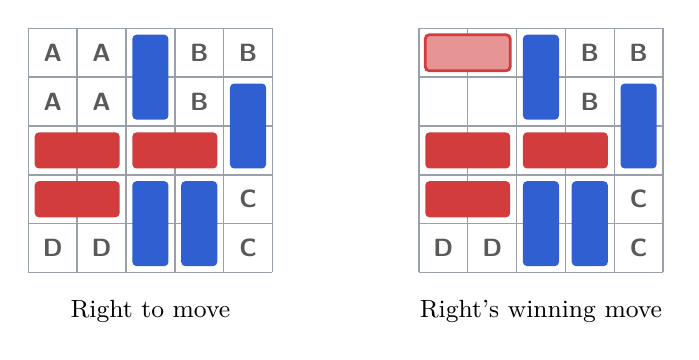
\begin{tikzpicture}[scale=0.62]
  \begin{scope}
    \grid{5}{5}
    \vd{1}{3} \vd{2}{5} \vd{4}{3} \vd{4}{4}
    \hd{3}{1} \hd{3}{3} \hd{4}{1}
    \lab{1}{1}{A}\lab{1}{2}{A}\lab{2}{1}{A}\lab{2}{2}{A}
    \lab{1}{4}{B}\lab{1}{5}{B}\lab{2}{4}{B}
    \lab{4}{5}{C}\lab{5}{5}{C}
    \lab{5}{1}{D}\lab{5}{2}{D}
    \node[font=\small] at (2.5,-5.8) {Right to move};
  \end{scope}
  \begin{scope}[xshift=8cm]
    \grid{5}{5}
    \vd{1}{3} \vd{2}{5} \vd{4}{3} \vd{4}{4}
    \hd{3}{1} \hd{3}{3} \hd{4}{1}
    \fill[rightc!55] (0.13,-0.87) rectangle (1.87,-0.13);
    \draw[rightc, line width=1pt, rounded corners=1.5pt] (0.13,-0.87) rectangle (1.87,-0.13);
    \lab{1}{4}{B}\lab{1}{5}{B}\lab{2}{4}{B}
    \lab{4}{5}{C}\lab{5}{5}{C}
    \lab{5}{1}{D}\lab{5}{2}{D}
    \node[font=\small] at (2.5,-5.8) {Right's winning move};
  \end{scope}
\end{tikzpicture}
\caption{Left: regions A ($2\times2$), B (L-tromino), C (vertical pair) and D (horizontal pair).
Right: the only winning move for Right, horizontally in region A.}
\end{figure}

\begin{center}
$\underbrace{\pm1}_{\text{A}} \;+\; \underbrace{*}_{\text{B}} \;+\; \underbrace{1}_{\text{C}}
\;+\; \underbrace{(-1)}_{\text{D}} \;=\; \pm1 + *$.
\end{center}

\noindent The sum $\pm1+*$ is a first-player win, and it is Right's turn, so Right wins with
correct play.  The question is \emph{where} Right should move:

\begin{itemize}
  \item \textbf{In A (correct).}  A becomes a horizontal pair, $-1$.  The total is $-1+*$,
        which is negative, so Right wins whatever Left does.
  \item \textbf{In B (loses).}  Taking the $*$ leaves $\pm1+1-1=\pm1$ with Left to move.  Left
        plays in A and wins.
  \item \textbf{In D (loses).}  Using up his own spare move leaves a position worth
        $\game{2*}{*}$, which is positive: Left wins.
\end{itemize}

CGSuite gives the same analysis: the position's canonical value is $\pm(1*)=\pm1+*$, and
Right's four options have values $-1*,\ -1*,\ \pm1,\ \game{2*}{*}$.

\begin{keybox}[title=Strategy in one sentence]
Do not waste spare moves (integers) and do not grab small values like $*$ while a \emph{hot}
region is still open: play where moving first gains the most.  That is the region with the
highest \emph{temperature}, here the $2\times2$ square with temperature $1$.
\end{keybox}

\section{Who wins on rectangular boards?}
\label{sec:boards}

Boards are given as \emph{rows} $\times$ \emph{columns}.  Results for small boards come from
CGSuite.  Results for large boards come from computer searches published in the literature,
collected in Nowakowski's list of unsolved problems (2025, problem B11).

\begin{center}
\begin{tabular}{@{}lll@{}}
\toprule
Board & Value & Winner \\
\midrule
$1\times n$, $n\ge2$ & $-\lfloor n/2\rfloor$ & Right (Left has no move) \\
$2\times2$, $3\times3$ & $\pm1$ & first player \\
$2\times3$ & $\game{2}{-\tfrac12}$ & first player \\
$3\times2$ & $\game{\tfrac12}{-2}$ & first player \\
$2\times4$ & $\{\{2\mid0\}\mid0\}$, a tiny negative value & Right \\
$4\times2$ & $\{0\mid\{0\mid-2\}\}$, a tiny positive value & Left \\
$2\times5$ & $\tfrac12$ & Left \\
$3\times4$ & $-\tfrac32$ & Right \\
$4\times3$ & $\tfrac32$ & Left \\
$4\times4$ & $\pm(\ldots)$, complicated & first player \\
\midrule
$8\times8$ & & first player (Breuker, Uiterwijk, van den Herik 2000) \\
$10\times10$ & & first player (Bullock 2002) \\
\bottomrule
\end{tabular}
\end{center}

Uiterwijk's solvers have settled many larger boards, for example whole families such as
$2k\times n$ for $n=3,5,7,9,11$ (Left wins).  Most boards, though, are known only by their
winner, not by their exact value.

\section{Why mathematicians care: open problems}

Domineering is a standard test case for combinatorial game theory.  It is easy to state, but
its values are rich.  Some questions that are still open (problem numbers from Nowakowski,
\emph{Unsolved problems in combinatorial games}, Games of No Chance 6, 2025):

\begin{itemize}
  \item \textbf{How hot can it get?}  All known positions have temperature at most $2$.  A
        position of value $\pm2*$ reaches it.  It is conjectured that $2$ is the maximum (the
        \emph{boiling point} of Domineering, E20, B11).
  \item \textbf{Which nimbers occur?}  Positions of value $*2$ and $*3$ are known.  The first
        $*2$ is due to Drummond-Cole; Uiterwijk and Barton found ones reachable from an empty
        board.  Whether $*4$ can occur is open (E6, E17).
  \item \textbf{Exact values of whole families.}  The value of $2\times n$ boards is known only up
        to an infinitesimal (``ish''), and the $3\times n$ and $4\times n$ families are open
        (B11).
  \item \textbf{Variants.}  Tromineering uses $1\times3$ pieces, and misère Domineering is the
        version where the player who cannot move wins.  Both are only partly analysed.
\end{itemize}

\section{Try it yourself}

CGSuite (\url{https://www.cgsuite.org}) computes Domineering values.  In a position string,
\texttt{.}\ is an empty square, \texttt{\#} is a filled square and \texttt{|} ends a row:

\begin{keybox}
\small\ttfamily
> game.grid.Domineering("..|..").CanonicalForm\\
+-1\\
> game.grid.Domineering("..\#..|..\#.\#|\#\#\#\#\#|\#\#\#\#.|..\#\#.").CanonicalForm\\
+-(1*)\\
> game.grid.Domineering(".....|.....").CanonicalForm\\
1/2
\end{keybox}

\paragraph{Further reading.}
\begin{itemize}[leftmargin=1.2em]
  \item M.\,H. Albert, R.\,J. Nowakowski, D. Wolfe, \emph{Lessons in Play}, A\,K Peters, 2007,
        ch.~1.  This is the standard gentle introduction and starts with Domineering.
  \item E.\,R. Berlekamp, J.\,H. Conway, R.\,K. Guy, \emph{Winning Ways for Your Mathematical
        Plays}, vol.~1.
  \item E.\,R. Berlekamp, Blockbusting and Domineering, \emph{J. Combin. Theory A} 49 (1988).
  \item A.\,N. Siegel, \emph{Combinatorial Game Theory}, AMS Graduate Studies in Mathematics
        146, 2013.
  \item R.\,J. Nowakowski, Unsolved problems in combinatorial games, \emph{Games of No Chance 6},
        MSRI Publ. 71, 2025, problems B11, E6, E17, E20.
\end{itemize}

\end{document}
